% !TEX encoding = UTF-8 Unicode
%oneside/twoside for the printer
\documentclass[a4paper,12pt,oneside,final,swedish]{extarticle}
%article vs. extarticle
%Paket
%\usepackage[latin1]{inputenc}	%å,ä,ö
\usepackage[utf8]{inputenc}
\usepackage[T1]{fontenc}
\usepackage{graphicx}
\usepackage{subcaption}
\usepackage{times}			%typsnitt times kanske
\usepackage[swedish]{babel}
\usepackage[affil-it]{authblk}
\usepackage{geometry}	%lets you customize the page size
\usepackage{hyperref}
\usepackage[ruled,vlined]{algorithm2e} %,vlined
\usepackage{algpseudocode}% http://ctan.org/pkg/algorithmicx
\usepackage{amsmath}

\geometry{
 margin=20mm
} 

\usepackage{fancyhdr} %include this to customize headers/footers
\usepackage{titling}

% Algoritm
\renewcommand{\algorithmcfname}{Algoritm}% Afrikaans "Algorithm"
\newlength\marincrease

%test \paragraph -subsubsub
\makeatletter
\renewcommand\paragraph{\@startsection{paragraph}{4}{\z@}%
            {-2.5ex\@plus -1ex \@minus -.25ex}%
            {1.25ex \@plus .25ex}%
            {\normalfont\normalsize\bfseries}}
\makeatother
\setcounter{secnumdepth}{4} % how many sectioning levels to assign numbers to
\setcounter{tocdepth}{4}    % how many sectioning levels to show in ToC

% För att sätta inventeringen för hela dokumentet
\setlength\parindent{0pt}
%\setlength{\parskip}{1cm plus4mm minus3mm}


%-------------------------------------------------------------Här börjar dokumentet 
\begin{document}
% Framsida
\author{Grupp 9\\\\Kalle Bladin\\Erik Broberg\\Emma Forsling Parborg\\Martin Gråd}
\affil{TNM085 - Modelleringsprojekt\\Linköpings Universitet}
\title{Simulering av Elastiska Material}
\clearpage\maketitle %genererar en separat titelsida
\thispagestyle{empty}
\date{2014-03-xx}
\affil{Linköpings Universitet}
\pagebreak
%\pagestyle{empty} %fancy, empty, plain, myheadings




%Sammanfattning
\begin{abstract}
\thispagestyle{empty}
\noindent Fysikbaserad animering av elastiska material kan sägas bestå av två skilda delar: fysikalisk simulering och grafikrendering. Materialen kan fysikaliskt beskrivas på flera olika sätt, men denna rapport är begränsad till att behandla endast en modell. Realismen i den simulering som presenteras är av stor vikt, varför fysikalisk korrekthet eftersträvas, och all beräkning grundar sig i vedertagna fysikaliska samband. För simuleringen undersöks två olika integreringsmetoder, Eulers stegmetod och Runge-Kuttas metod, och deras respektive för- och nackdelar med hänsyn till snabbhet och stabilitet.

\noindent \\De förstudier som presenteras härleder den ekvation som simuleringen bygger på. Denna grundar sig i sin tur på de fysikaliska samband som presenteras i Bakgrund. Förstudierna tar också upp modelleringen av det system som simuleras, och även de numeriska metoder som är implementerade. Resultaten från förstudierna valideras och ligger som grund för den slutgiltiga implementeringen.

\noindent \\De slutliga simuleringar som presenteras visar att den valda modellen kan efterlikna ett antal olika material och deras egenskaper. Utritningen sker med en bestämd frekvens, och noggrannheten i integreringarna bestäms utifrån denna. Undersökningen av integreringsmetoderna visar att Eulers stegmetod är att föredra i detta sammanhang.
\hfill
\end{abstract}
\pagebreak 

%Innehållsförteckning, Figurförteckning & Tabellförteckning
\tableofcontents  % chapter with the table of contents
\addtocontents{toc}{\protect\thispagestyle{empty}}
\listoffigures    % chapter with the list of figures
\addtocontents{lof}{\protect\thispagestyle{empty}}
\listoftables     % chapter with the list of tables
\addtocontents{lot}{\protect\thispagestyle{empty}}

%-----------------------------------------------------------
%\pagestyle{plain}
\pagebreak
\pagestyle{plain}
\setcounter{page}{1}

%Inledning
\section{Inledning}
Simulering av elastiska material används flitigt i moderna fysikmotorer. Dessa kan användas både i datorspel och animeringsmjukvara där realism är en viktig faktor. Med hjälp av simulering behöver inte en animatör explicit hantera vissa rörelser hos objekten.
\subsection{Bakgrund}
Grundidén till systemet ligger i tidigare presenterade studier kring liknande ämnen. Partikelsystem i sin helhet kan anta många olika former. Elastiska material täcker flera sådana då det går att göra en väldigt generell modell för att simulera många olika material. Bristen med många fysikaliska simuleringar är att modellen endast täcker ett väldigt specifikt område som till exempel tygsimulering eller endast hårda material.
\subsection{Syfte}
Denna rapport syftar till att undersöka hur verklighetstrogna simuleringar av elastiska material kan göras i tre dimensioner med hjälp av mass-fjäder-dämparsystem. Simuleringarna som demonstreras är menade att kunna göras i realtid, och erbjuda en användare viss interaktion. Det är även viktigt att modellen ska kunna täcka många olika delar av newtonsk fysik; allt från elastiskt tyg till tärningskast med hårda tärningar.

%Metod
\section{Metod}
\subsection{Förstudier}
I förstudierna ingick dels framtagandet av en kraftekvation, dels utvecklingen av MSD-system i en och två dimensioner. Detta grundar sig i den fysikaliska modelleringen samt numerisk lösning av differentialekvationer. Som verktyg användes MATLAB för att få en visuell återkoppling på kraftekvationen, med hjälp av programmets inbyggda renderingsfunktion.
\subsubsection{Fysikalisk modellering}
En modell som kan användas för simulering av elastiska material är ett så kallat ''mass spring damper system'' (Gelenbe, Lent \& Stakellari 2012) eller MSD-system; en modell som beskrivs av partiklar sammankopplade med fjädrar och dämpare.\\
\begin{figure}[h!]
  \begin{center}
    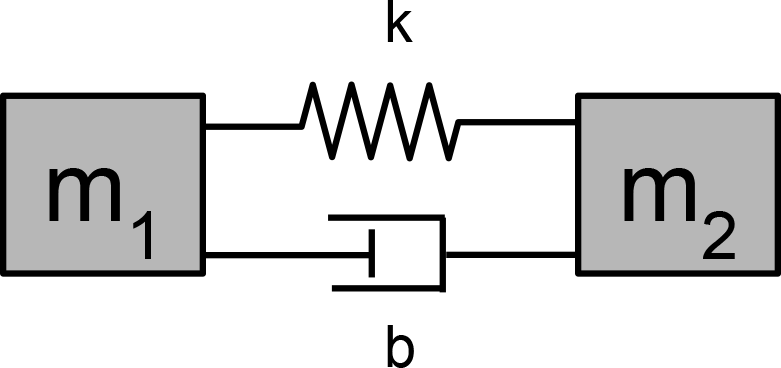
\includegraphics[width=5cm]{Bilder/simple1D.png} 
  \end{center}
  \caption{Två partiklar med massorna $m1$ och $m2$, sammankopplade med en fjäder med fjäderkonstanten $k$ och en dämpare med dämparkonstanten $b$.}
  \label{m1m2::nonfloat}
\end{figure}
\\Det enkla systemet i Figur \ref{m1m2::nonfloat} utgör grunden för den struktur som används i detta projekt. Genom att utöka systemet med partiklar och samma typ av kopplingar, kan många olika material och former beskrivas, exempelvis tyg, gelé, skumgummi eller liknande. Beroende på parametrarna fjäderkonstanter, dämparkonstanter, massor och fjäderlängder kan realistiska simuleringar av dessa material uppnås.
\\\\Som bakgrund till den fysikaliska modellen låg de grundläggande rörelse- och kraftlagarna som beskrevs av Newton (Halliday 2007). Newtons andra lag anges i (2),

\begin{equation}
	{ \mathbf F }_{ k }(t)=-k(\Delta x(t)-{ l }_{ o })
\end{equation}
där F(t) är den resulterande kraften på en partikel, x’’(t) är partikelns acceleration, m är partikelns massa och t är tidsvariabeln. Newtons tredje lag summeras i ett citat:
Newtons tredje lag summeras i ett citat:
\begin{quote}\begin{center}\textit{''If A puts a force on B, then B puts a force on A, and the two forces are equal in magnitude and have opposite direction.''} (Halliday 2007)\end{center}\end{quote}
Fjädrarna modellerades med Hookes lag som anges i (3),

\begin{equation}
	{ F }_{ k }(t)=-k(\Delta x(t)-{ l }_{ o })
\end{equation}

där Fk(t) är kraften som fjädern uträttar, k är fjäderkonstanten, l0(t) är fjäderns utsträckning, och l0 är fjäderns vilolängd.
\\\\Dämparna modellerades utifrån ekvation 4,

\begin{equation}
{ F }_{ b }(t)=-bl'(t)
\end{equation}

där Fb(t) är kraften som dämparen uträttar, b är dämparkonstanten och l är fjäderns utsträckning.

\subsubsection{Numerisk lösning av differentialekvationer}
Som bakgrund till simuleringen och därmed numerisk integrering låg Eulers stegmetod och Runge-Kuttametoden (Ljung \& Glad 2003). Nedanstående ekvationer beskriver numerisk integrering som krävs för lösning av första ordningens differentialekvationer, se (5).

\begin{equation}
\mathbf x'(t)=\mathbf f(t,\mathbf x(t))
\end{equation}

Här är x(t) den sökta funktionen, och dess derivata är en funktion av tiden t samt funktionen x(t) själv.
\paragraph{Euler}%subsubsub
Eulers stegmetod för att lösa första ordningens differentialekvationer beskrivs i (6),

\begin{equation}
\mathbf x(t+h)=\mathbf x(t)+\mathbf f(t,\mathbf x(t))h
\end{equation}

där h är tidssteget, och f fås från differentialekvationen. För att hitta funktionsvärdet vid tidpunkten t+h, alltså h tidsenheter efter det föregående, används funktionen f från differentialekvationen samt funktionsvärdet i det nuvarande steget, x(t). Efter ett givet startvärde kan en numerisk lösning tas fram genom stegning med jämna intervall.
\paragraph{Runge Kutta}%subsubsub
Att lösa differentialekvationen med Runge-Kuttametoden innebär att flera derivator beräknas vid olika tidssteg. Detta ger en mer korrekt integrering jämfört med Eulers stegmetod (Jönsson 2010). Detta innebär att funktionen f har olika argument för att beräkna förändringshastigheterna k1, ..., k4. Funktionsvärdet i tidpunkten t+h baseras på en viktad summa av förändringshastigheterna enligt (7) nedan.

\begin{equation}
\begin{split}
\mathbf x(t+h)=\mathbf x(t)+\frac { 1 }{ 6 } ({ k }_{ 1 }+2{ k }_{ 2 }+2{ k }_{ 3 }+{ k }_{ 4 })
\\ där
\\ \mathbf{ k }_{ 1 }=h\mathbf f(t,\mathbf x(t))
\\ \mathbf{ k }_{ 2 }=h\mathbf f(t+h/2,\mathbf x(t)+\mathbf { k }_{ 1 }/2)
\\ \mathbf{ k }_{ 3 }=h\mathbf f(t+h/2,\mathbf x(t)+\mathbf{ k }_{ 2 }/2)
\\ \mathbf{ k }_{ 4 }=h\mathbf f(t+h,\mathbf x(t)+\mathbf{ k }_{ 3 })
\end{split}
\end{equation}

Funktionen f har här givits olika argument som leder till de olika förändringshastigheterna k1, …, k4. Med vikterna satta enlig (BÖS7) ovan ges i detta fall Runges metod (Jönsson 2010).
\subsubsection{Kraftekvation}
\subsubsection{Utveckling av MSD-system}
\paragraph{En dimension}
Då det enkla systemet med två sammankopplade partiklar utökades med fler partiklar och kopplingar, krävdes en mer överskådlig notation för att beskriva systemet. 
I figur \ref{2D_simple::nonfloat} nedan introduceras den nya notationen av ett system med två sammankopplade massor.

\begin{figure}[h!]
  \begin{center}
    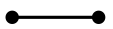
\includegraphics[width=3cm]{Bilder/2D_simple.png} 
  \end{center}
  \caption{Två sammankopplade partiklar}
  \label{2D_simple::nonfloat}
\end{figure}
\noindent I MATLAB utvecklades först ett MSD-system i en dimension, där partiklar sammankopplades i serie enligt Figur \ref{simple1D4::nonfloat} nedan.
\begin{figure}[h!]
  \begin{center}
    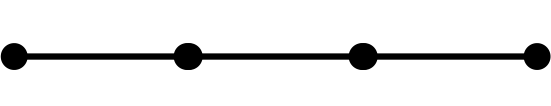
\includegraphics[width=6cm]{Bilder/simple1D4.png} 
  \end{center}
  \caption{Fyra sammankopplade partiklar i serie}
  \label{simple1D4::nonfloat}
\end{figure}

\noindent Genom att simulera detta system med Euler-metoden samt undersöka hur partiklarnas positioner förändrades över tid, kunde implementeringen av den framtagna kraftekvationen enkelt verifieras.

\paragraph{Två dimensioner}
Nästa steg i utvecklingen av MSD-systemet var att implementera det i två dimensioner. 
Detta innebar en övergång från skalärer till vektorer i de framtagna ekvationerna.
\pagebreak


\noindent För att kunna generera godtyckligt stora MSD-system krävdes en regel för hur partiklarna skulle kopplas ihop med varandra. Två exempel på en partikels möjliga kopplingar visas i Figur \ref{2D_Neighbors::nonfloat} nedan.

\begin{figure}[h]
  \begin{minipage}[h!]{.5\linewidth}
    \centering
    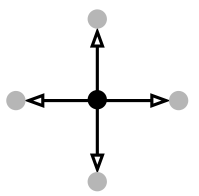
\includegraphics[width=4cm]{Bilder/2D_4Neighbors.png} 
    \subcaption{Partiklar med fyra kopplingar}\label{fig:1a}
  \end{minipage}
  \begin{minipage}[h!]{.5\linewidth}
    \centering
    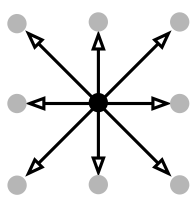
\includegraphics[width=4cm]{Bilder/2D_8Neighbors.png} 
    \subcaption{Partiklar med åtta kopplingar}\label{fig:1b}
  \end{minipage}
  \caption{Två olika sätt att koppla samman partiklar}
  \label{2D_Neighbors::nonfloat}
\end{figure}

\noindent \\Kopplingsregeln i Figur \ref{2D_Neighbors::nonfloat} a) ger upphov till en struktur som är instabil. Detta beror på att kopplingarnas ändpunkter endast har en position; ingen riktning eller orientering. Detta medför att strukturen kollapsar, vilket visas i Figur \ref{2D_Instabil::nonfloat}.

\begin{figure}[h!]
  \begin{center}
    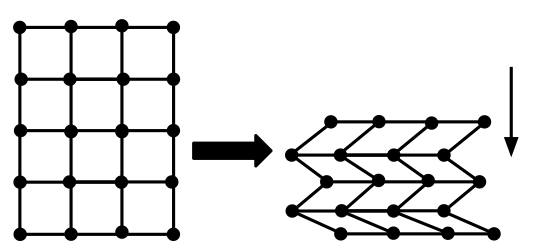
\includegraphics[width=8cm]{Bilder/2D_Instabil.png} 
  \end{center}
  \caption{Instabil struktur ges av kopplingsregeln i Figur \ref{2D_Neighbors::nonfloat} a) }
  \label{2D_Instabil::nonfloat}
\end{figure}

\noindent Med regeln enligt Figur \ref{2D_Neighbors::nonfloat} b) erhålls däremot en struktur som är mer stabil, men fortfarande inte alltför komplex. Att materialet inte skulle kollapsa var en förutsättning för att elastiska material skulle kunna modelleras på ett trovärdigt sätt. Detta motiverade valet att använda kopplingar enligt figur \ref{2D_Neighbors::nonfloat} b). Strukturen som ges med denna regel redovisas i Figur \ref{2D_stabil::nonfloat} nedan.

\begin{figure}[h!]
  \begin{center}
    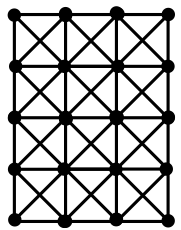
\includegraphics[width=3cm]{Bilder/2D_stabil.png} 
  \end{center}
  \caption{Stabil struktur ges av kopplingsregeln i Figur \ref{2D_Neighbors::nonfloat} b)}
  \label{2D_stabil::nonfloat}
\end{figure}

\subsubsection{Indexering av partiklar och kopplingar}
Ett stort problem som kopplingsmetoden i ovanstående stycke medförde var vilka partiklar som skulle höra till varje koppling. För att detta skulle kunna lösas för godtyckligt stora objekt, behövdes ett systematiskt sätt att tilldela kopplingarna deras partiklar. Detta löstes med en funktion som utifrån index till en viss koppling gav indexar till de två partiklar som den kopplade samman. Genom att låta funktionen genomlöpa alla kopplingar innan simuleringen genomfördes kunde indexeringen användas för att finna de rätta konstanterna (massorna) och variablerna (positionerna och hastigheterna) för de sammankopplade partiklarna. En liknande funktion implementerades för att finna triangelindexar som användes för renderingen.

\subsubsection{Interaktion med omgivning}
Gravitation simulerades genom att den globala tyngdaccelerationen på \begin{math}9.82 m/s^2 \end{math} adderades på samtliga partiklars acceleration i samband med beräkningen av krafterna. Tillsammans med detta implementerades hantering av kollision med ett markplan för att materialets beteende skulle kunna studeras under bekanta förhållanden (se Figur \ref{blaa::nonfloat}). Kollisionen implementerades genom en enkel algoritm.

  %Algoritm 1: Kollision
\begin{algorithm}[H]
  \For{varje partikel $i$}{
    \If{partikeln befinner sig under kollisionsplanet:}{
%    spegla hastighetsvektorn i kollisionsplanet\;
 %   projicera positionsvektorn upp på kollisionsplanet\;
 %   multiplicera den komponent av hastighetsvektorn som är parallell med kollisionsplanet med en friktionskoefficient\;
%    multiplicera den komponent av hastighetsvektorn, som är ortogonal med\\ kollisionsplanet, med en elasticitetskoefficient\;
    
      \begin{itemize}
      \item Spegla i:s hastighetsvektor i kollisionsplanet, se Figur \ref{kol3}.\
      \item Ortogonalprojicera i:s positionsvektor upp på kollisionsplanet, se Figur \ref{kol3}.\
      \item Multiplicera den komponent av i:s hastighetsvektor som är parallell med\\ kollisionsplanet med en friktionskoefficient, se Figur \ref{kol4}\
      \item Multiplicera den komponent av i:s hastighetsvektor, som är ortogonal med\\ kollisionsplanet, med en elasticitetskoefficient, se Figur \ref{kol4}.\
    \end{itemize}
    }
  }
\caption{Kollision\label{alg1}}
\end{algorithm}
  %Bilder
\begin{figure}[h]
  \begin{minipage}[b]{.5\linewidth}
    \centering
    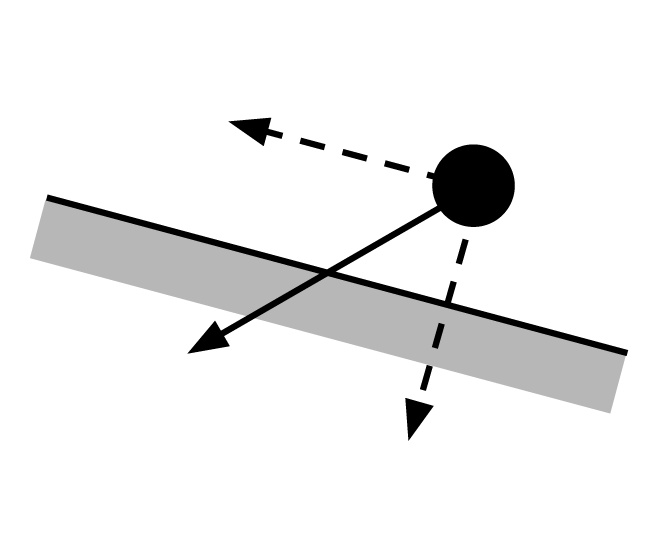
\includegraphics[width=4cm]{Bilder/kollision_01.png} 
    \subcaption{Partikeln rör sig mot kollisionsplanet.}\label{kol1}
  \end{minipage}
  \begin{minipage}[b]{.5\linewidth}
    \centering
    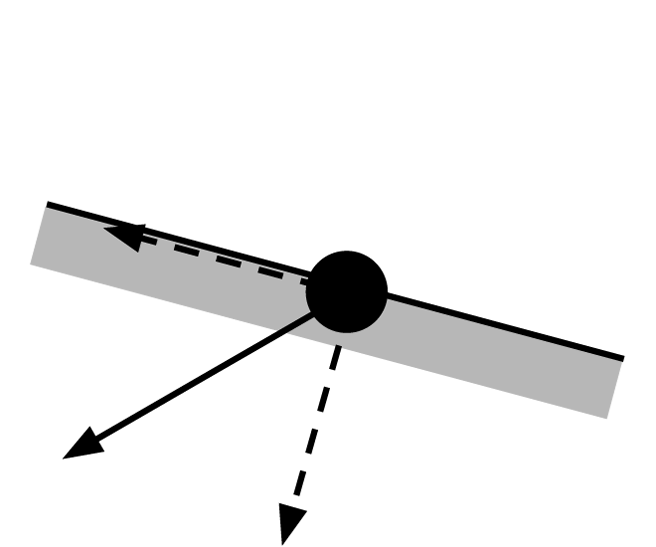
\includegraphics[width=4cm]{Bilder/kollision_02.png} 
    \subcaption{Partikeln har kolliderat med planet.}\label{kol2}
  \end{minipage}
  \begin{minipage}[b]{.5\linewidth}
    \centering
    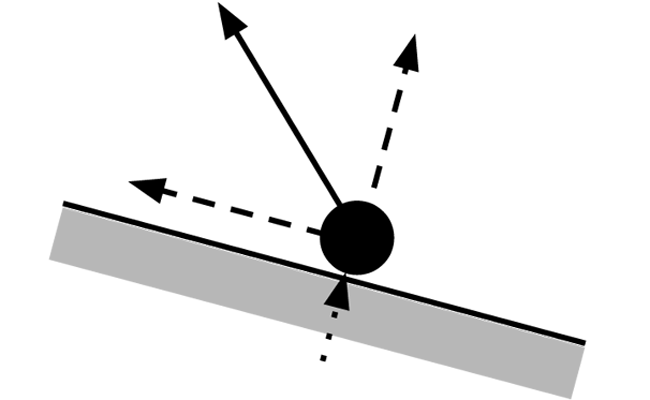
\includegraphics[width=4cm]{Bilder/kollision_03.png} 
    \subcaption{Partikelns position och hastighetsvektor ändras.}\label{kol3}
  \end{minipage}
  \begin{minipage}[b]{.5\linewidth}
    \centering
    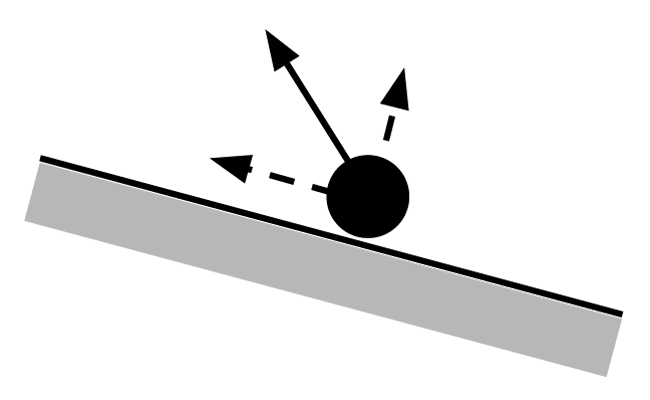
\includegraphics[width=4cm]{Bilder/kollision_04.png} 
    \subcaption{Komponenterna multipliceras med deras respektive koefficient.}\label{kol4}
  \end{minipage}
  \caption{Två olika sätt att koppla samman partiklar}
  \label{blaa::nonfloat}
\end{figure}

\subsubsection{Implementering av kraftekvationen}
Att implementera kraftekvationen för varje partikel i ett MSD-system enligt (KRAFTEKV), innebär att kraftvektorn till varje partikel $i$ beräknas. Med denna kraftvektor kan i sin tur accelerationen beräknas för varje partikel enligt (DIFFEKV). I detta projekt undersöktes två algoritmer för detta ändamål.\\\\
%Algorithm 2: baserad på massorna
\begin{algorithm}[H]
  \For{varje partikel $i$}{
    \For{varje partikel $j$, som är kopplad till $i$}{
	f = kraften på i från kopplingen mellan i och j\;
	F[i] += f\;
    }
    beräkna accelerationen genom att dividera F[i] med i:s massa\;
    nollställ F[i]\;
  }
\caption{Algoritm baserad på partiklar\label{alg2}}
\end{algorithm}
%Algorithm 3: baserad på kopplingarna mellan massorna
\begin{algorithm}[H]
  \For{varje koppling $c$ (där $c$ är kopplingen mellan partikel $i$ och $j$) :}{
 	f = kraften på i från koppling c\;
	F[i] += f\;
	F[j] -= f\;
  }
  \For{varje partikel $i$}{
      beräkna accelerationen genom att dividera F[i] med i:s massa\;
      nollställ F[i]\;
  }
\caption{Algoritm baserad på kopplingarna mellan partiklar\label{alg3}}
\end{algorithm}
\noindent \\\\I Algoritm \ref{alg2} utnyttjas det faktum att en koppling påverkar dess två ändpunkter med lika stora krafter, med enda skillnaden att de är motriktade varandra. På så sätt reduceras antalet beräkningar av kraftekvationen till hälften, vilket motiverade beslutet att Algoritm \ref{alg2} användes i detta projekt. Läsaren kan övertyga sig själv om att antalet beräkningar av kraftekvationen halveras genom att betrakta följande enkla MSD-system.
\begin{figure}[h!]
  \begin{center}
    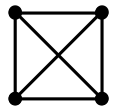
\includegraphics[width=3cm]{Bilder/2D_2x2.png} 
  \end{center}
  \caption{Enkelt system med fyra hopkopplade partiklar}
  \label{enkelfyra::nonfloat}
\end{figure}
\\I Figur \ref{enkelfyra::nonfloat} har varje partikel tre hopkopplade grannar. Det totala antalet grannar blir således tolv, vilket är dubbla antalet kopplingar, som är sex.

\subsection{Implementering}
Programkoden från Matlab porterades till C++ där systemet utvecklades vidare. Fördelen med C++ är att det är snabbt, objektorienterat (Skansholm 2012), samt att en utvecklare får mer kontroll, inte minst över grafikprogrammeringen. Grafikprogrammeringen gjordes med OpenGL som är plattformsoberoende och ger utvecklaren möjlighet att använda hårdvaruaccelererad grafik (Gortler 2012).
\subsubsection{Grundläggande systemarkitektur}
Att övergå till ett objektorienterat system innebar att en systemarkitektur behövde tas fram. 
För att ge en grundläggande förståelse av systemarkitekturen beskrivs denna med ett blockdiagram där de primära modulerna är separerade från varandra. 
Se Figur \ref{systemark::nonfloat}.
\begin{figure}[h!]
  \begin{center}
    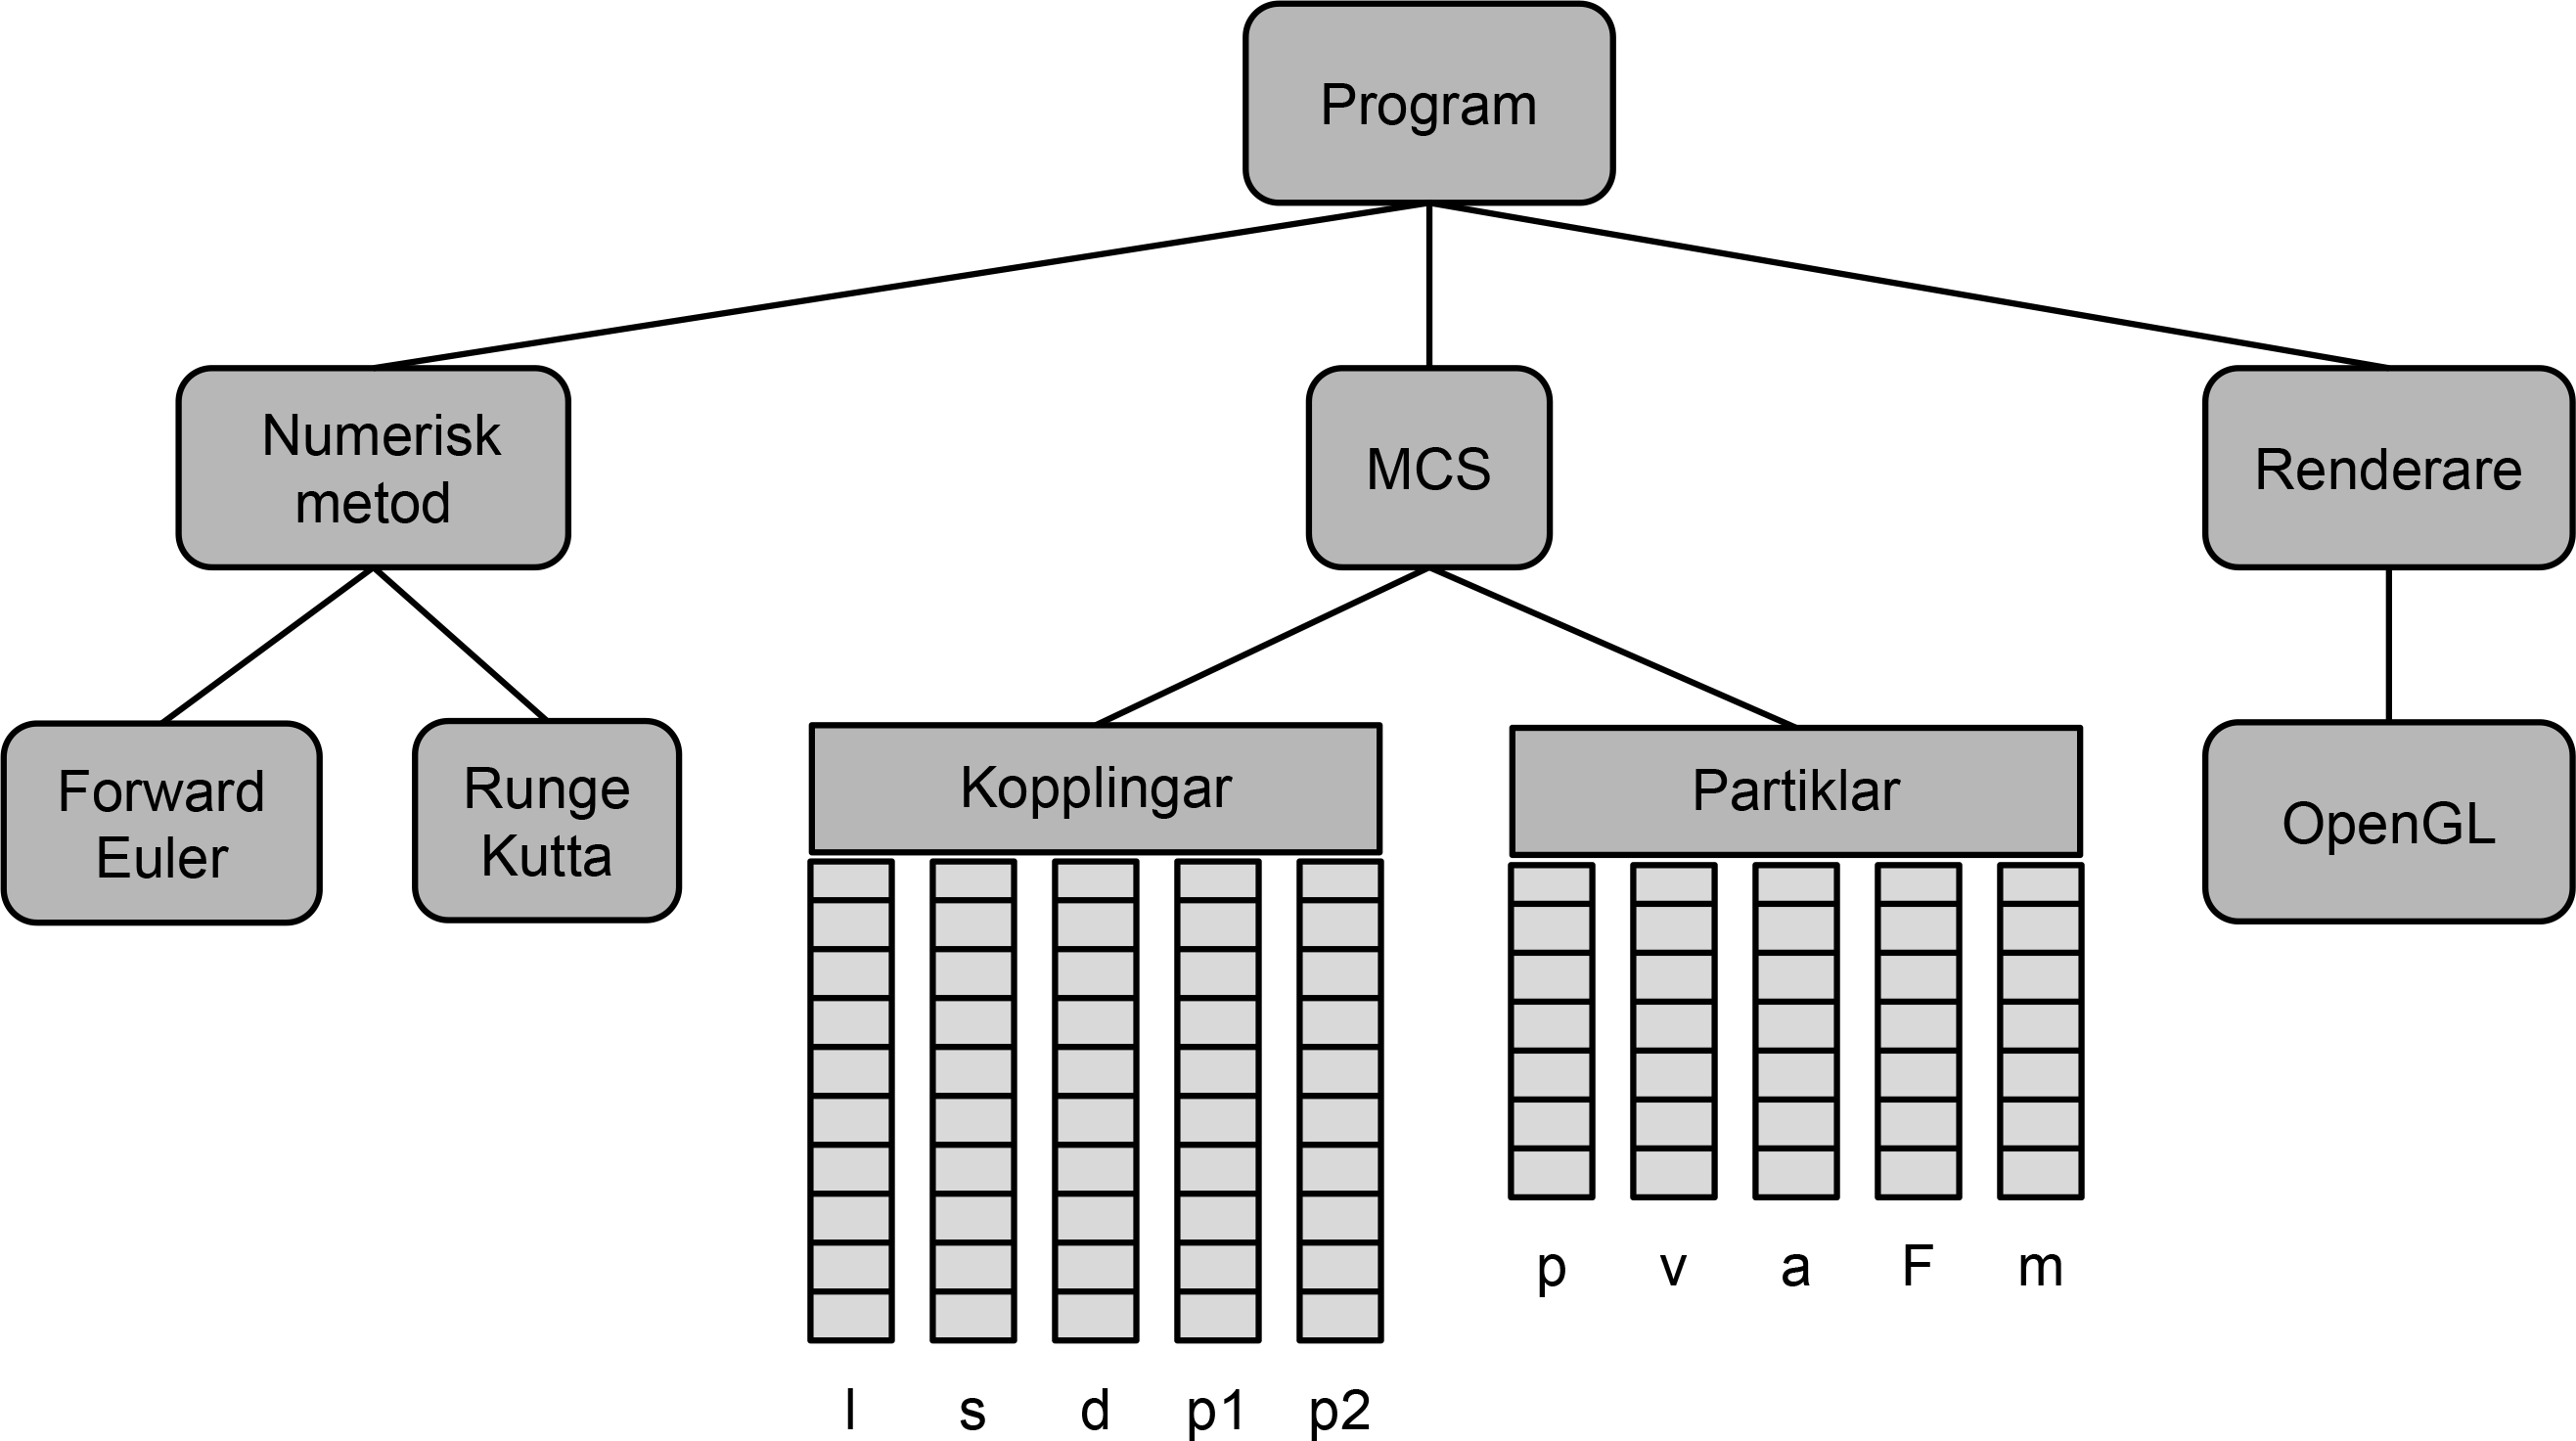
\includegraphics[width=16cm]{Bilder/Arkitektur.png} 
  \end{center}
  \caption{Övergripande systemarkitektur}
  \label{systemark::nonfloat}
\end{figure}
\\Klassen MCS (Mass Connection System) är den klass som lagrar all huvudsaklig data. Den innehåller samtliga partiklar och kopplingar för ett system.
\\\\Alla partiklar identifieras med ett index, och definieras av följande information:
\begin{itemize}
  \item p, position
  \item v, hastighet
  \item a, acceleration
  \item F, total momentan kraftpåverkan
  \item m, massa
\end{itemize}
Samtliga kopplingar identifieras med ett index, och definieras av följande information:
\begin{itemize}
  \item l, vilolängd
  \item k, fjäderkonstant
  \item b, dämparkonstant
  \item p1, index till den partikel som utgör kopplingens ena ändpunkt
  \item p2, index till den partikel som utgör kopplingens andra ändpunkt
\end{itemize}
Vad som också framgår i Figur Figur \ref{systemark} är att all numerisk integrering beräknas i en separat modul vilket gjorde det enkelt att ändra integreringsmetod vid behov, då den var oberoende av resten av systemet.
%OBS OBS OBS fixa ekvationer!!!!! här under
\subsubsection{Implementering av numeriska integreringsmetoder}
Efter att accelerationen för varje partikel hade beräknats genom (BLAHA (den med g)), approximerades deras positioner med en numerisk stegmetod. Den numeriska integreringen gjordes två gånger per tidssteg, då det var en andra ordningens differentialekvation som skulle lösas. Se ekvation (DIFF EKV). Nedan beskrivs hur de två olika integreringsmetoderna i systemet implementerades.
\paragraph{Eulers stegmetod} 
Med ett givet tidssteg h beräknades den nya hastigheten utifrån accelerationen a. Hastigheten användes i sin tur för att beräkna den nya positionen. 034i342
	\begin{equation} 
	v = v_old + a*h;		%OBS!!!! ATT FIXA TILL 
	p = p_old + v*h; 
	\end{equation}
\paragraph{Runge Kutta}
En algoritm för att simulera MSD-systemet med Runge-Kutta implementerades. Genom att kalla på kraftekvationen med olika steglängder kunde värdena $k1$, ..., $k4$ beräknas. Här användes en specifik variant av Runge-Kuttametoden, nämligen Runges variant, med vikterna \begin{math} w_1 = 1, w_2 = 3, w_3 = 3, w_4 = 1 \end{math}.
\subsubsection{Rendering}
För att rendera MSD-systemet skickades hörnpunkter, en triangellista, en lista med färger för varje hörnpunkt samt en lista med normaler till grafikkortet via OpenGL. På grafikkortet kunde det elastiska materialet färgas. Dessutom kunde Phong shading implementeras för att simulera att modellen belyses från en viss riktning. Denna rendering gjordes 60 gånger per sekund.
\subsection{Stabilitets- och prestandatest}
För att jämföra stabiliteten i de två numeriska metoderna gjordes en enkel undersökning. För ett givet MSD-system och en viss steglängd hittades metodernas stabilitetsgränser genom en stegvis ökning av fjäderkonstanterna.
\\\\När stabilitetsgränser för de numeriska metoderna hade bestämts, behövde en avvägning mellan fysikalisk noggrannhet och renderingsfrekvens göras. För att simuleringen skulle kunna erbjuda responsiv interaktion och jämn animering togs beslutet att antalet tidssteg i simuleringen skulle anpassas för att uppnå en bestämd utritningsfrekvens.
\\\\För att jämföra de två olika numeriska integreringsmetoderna som har implementerats utfördes ett stabiltets- och prestandatest. Först användes Runge-Kuttametoden med ett visst antal tidssteg per utritning så att en jämförbar utritningsfrekvens erhölls. Därefter undersöktes hur många tidssteg per utritning som krävdes för att Eulers metod skulle ge samma utritningsfrekvens. Simuleringarna tog då lika lång tid att genomföra och stabilitetsgränsen kunde kontrolleras genom att öka fjäderkonstanterna eller dämparkonstanterna oberoende av varandra.
%Resultat
\section{Resultat}
Resultaten från förstudier och implementering presenteras nedan.
\subsection{Resultat från förstudier}
Resultatet från förstudierna i en dimension presenteras i Figur \ref{endim::nonfloat}. Här illustreras fem sammankopplade partiklars samverkan efter att en av dem har givits en förskjuten startposition. Den kraft som bildas av denna förskjutning kan ses påverka de andra partiklarna och fortplantas genom systemet över tid. Krafterna ses också dämpas och tillslut avta, vilket stabiliserar systemet.

\begin{figure}[h!]
  \begin{center}
    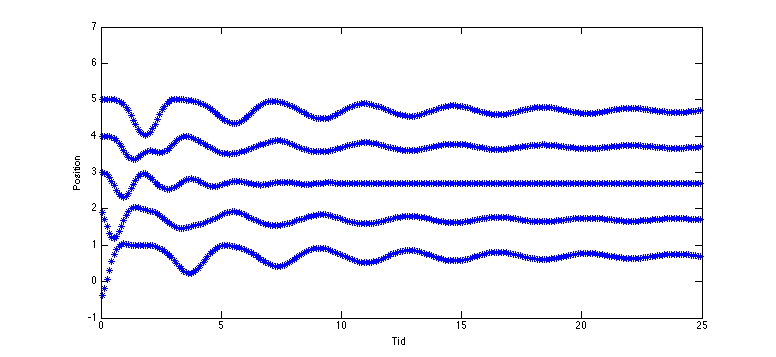
\includegraphics[width=16cm]{Bilder/1D_matlab.png} 
  \end{center}
  \caption{Endimensionellt MSD-system i MATLAB}
  \label{endim::nonfloat}
\end{figure}

\noindent \\I Figur \ref{tvådim::nonfloat} åskådliggörs resultatet av förstudierna i två dimensioner. Här illustreras ett 4x4 MSD-system som faller från sin startposition och därefter kolliderar med ett markplan.
Fjädrarnas inverkande krafter visualiseras genom att låta färgen bero på kopplingens längd. 
Kopplingen är grön i sitt viloläge och färgen går mot rött ju mer längden avviker från denna.

\begin{figure}[h!]
  \begin{center}
    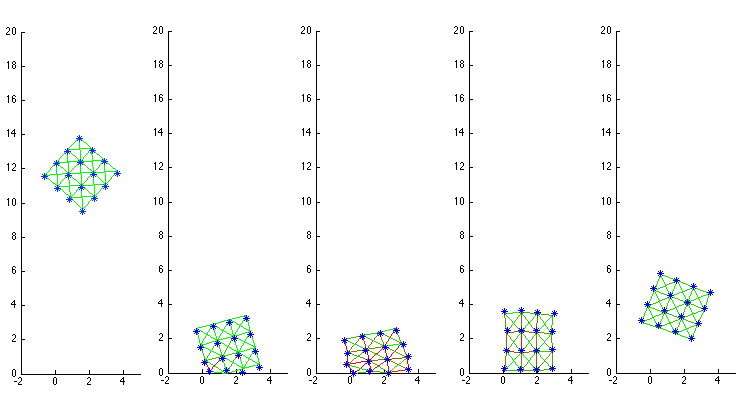
\includegraphics[width=16cm]{Bilder/boing.png} 
  \end{center}
  \caption{Tvådimensionellt 4x4 MSD-system i MATLAB}
  \label{tvådim::nonfloat}
\end{figure}

\subsection{Resultat från implementering}
I Figur (\ref{b1::nonfloat}) och (\ref{b2::nonfloat}) visas bilder från simuleringar av två olika material. Materialen skiljer sig åt både i form och parametervärden. Det första materialet har relativt höga fjäderkonstanter och låga dämparkonstanter, medan det andra materialets egenskaper är de motsatta.
\begin{figure} [h] 
 \begin{minipage}[b]{.5\linewidth}
    \centering
    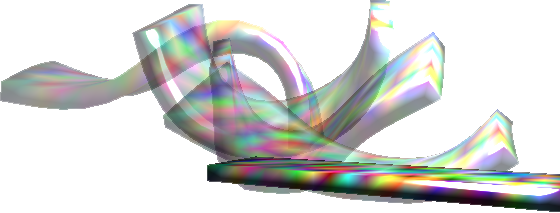
\includegraphics[width=8cm]{Bilder/Anim1.png} 
    \subcaption{}\label{b1::nonfloat}
  \end{minipage}
 \begin{minipage}[b]{.5\linewidth}
    \centering
    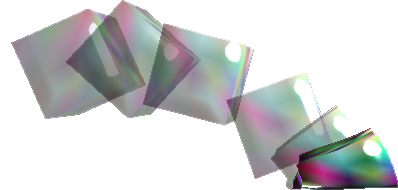
\includegraphics[width=8cm]{Bilder/Anim2.png} 
    \subcaption{}\label{b2::nonfloat}
  \end{minipage}
  \caption{Resultat från implementering}
  \label{res_imp::nonfloat}
\end{figure}


\subsection{Resultat från stabilitets- och prestandatest}
%Tabeller
Testet av stabilitetsgränser för de numeriska metoderna presenteras i Tabell \ref{table_example1} , och testet av stabilitet utifrån önskad prestanda presenteras i Tabell \ref{table_example2}.
\begin{table}[htbp]
    \caption{Erhållna resultat för en bestämd steglängd.}
    \label{table_example1}
    \begin{tabular*}{\hsize}{lllll}
      \hline %streck
       & \bfseries Fjäderkonstant (för marginell stabilitet)\\
      \hline
      \bfseries Runge Kutta: & xxx\\
      \bfseries Euler: & xxx\\
      \hline
    \end{tabular*}
\end{table}

\begin{table}[htbp]
    \caption{Erhållna resultat för ett bestämt antal utritningar per sekund.}
    \label{table_example2}
    \begin{tabular*}{\hsize}{lllll}
      \hline %streck
       & \bfseries Simuleringar per utritning & \bfseries Fjäderkonstant(för marginell stabilitet)\\
      \hline
      \bfseries Runge Kutta: & 7 & 40 000\\
      \bfseries Euler: & 44 & 2150000\\
      \hline
    \end{tabular*}
\end{table}
%Diskussion
\section{Diskussion}
Under projektets gång gjordes ett antal val. Dessa är val av numerisk metod, algoritm för kraftkvation, fjädersortering/indexering samt dämpare.

\noindent\\Den största anledningen till att Runge-Kuttametoden var mer beräkningstung var att mycket data behövde kopieras under simuleringen. Runge-Kuttametoden gav visserligen en mer korrekt simulering men eftersom det var kritiskt att med hög prestanda erhålla ett relativt stabilt system gjordes valet att använda Eulers metod i slutprodukten.

\noindent\\Valet av algoritm för kraftekvationen grundade sig i antalet gånger kraftekvationen behövde beräknas. Med Algoritm \ref{alg3} behövde beräkningen göras hälften så många gånger. Dock krävde algoritmen att partiklarna loopades igenom en gång efter det att krafterna hade beräknats för att applicera accerelationen på dem. Trots detta hölls antalet beräkningar på en lägre nivå för Algoritm \ref{alg3} än för Algoritm \ref{alg2}, varför Algoritm \ref{alg3} valdes för slutimplementeringen.

\noindent\\Vid skapande av MSD-systemet gjordes begränsningar i val av dämpare med enbart dynamisk friktion. Att införa andra ekvationer för hur dämparna modelleras skulle kunna vara en vidareutveckling av systemet. En möjlighet är att införa statisk friktion i dämparna för att simulera deformation i materialet så att det inte återfår sin ursprungliga form.

\noindent\\Vid utveckling av MSD-systemet underlättade MATLABs inbyggda renderingsfunktion. Med hjälp av den kunde kraftekvationen valideras utan att tid behövde spenderas på implementering av en egen renderingsfunktion. Med den tidiga visuella återkopplingen var felsökning lättare, vilket gav upphov till ett smidigare arbetsflöde och fokus kunde läggas på rätt del i början av arbetet.

\noindent\\En annan del av systemet som tål att diskuteras är hur andra former än rätblock skulle kunna ställas upp. Indexeringsfunktionen förutsätter att modellen är uppbyggd i rätblocksformation medan simuleringen i sig inte förutsätter något sådant. Fördelen är alltså att man kan implementera andra indexeringsfunktioner för att bygga upp modeller av andra former, som sfärer eller koner.

\noindent\\Indexeringsfunktionen i sig kunde också ha implementerats annorlunda för att göra arbetet med den lättare. I stället för en funktion som utifrån fjäderindex ger två partikelindexar kunde listan med partiklar loopas igenom vartefter en koppling kunde läggas till för partikelns alla grannar. Denna metod hade varit lättare att implementera men saknar fördelen att listan med kopplingar blir ordnad på ett systemetiskt sätt. Fördelen med den första metoden var att kopplingarna ordnades efter längderna, vilket underlättade proceduren att ändra dessa under körning. Möjligheten att veta exakt vilken koppling som tillhörde vilket index ger möjlighet till större kontroll.

\noindent\\Fortsatt utveckling av grafiken skulle främst vara införandet av texturer. Detta är en naturlig vidareutveckling då det skulle innebära införandet av en lista med UV-koordinater i stället för listan med färger som användes i renderingen. För detta skulle en ny indexeringsfunktion krävas för att ta fram vilken hörnpunkt som tillhör en viss UV-koordinat. Med texturer ges möjligheten att rendera mer verklighetstrogna och intressanta material. Rendering av andra element såsom markplan skulle också tillföra ett mervärde genom att förtydliga kollisionen med detta. Skuggkastning är också något grafiskt som skulle förtydliga interaktionen mellan materialet och markplan genom att ge en känsla för avstånd.


%Referenser
\section{Referenser}
Fausett, L.V , 2008, \textit{Applied Numerical Analysis Using Matlab}, Pearson Prentice Hall.

\noindent \\Gelenbe, E, Lent, R, Stakellari, G, 2012, \textit{Computer and Information Sciences II: 26th International Symposium on Computer and Information Sciences}, Springer-Verlag London Limited.

\noindent \\Gortler, S.J, 2012, \textit{Foundations of 3D Computer Graphics}, The MIT Press.

\noindent \\Halliday, D, 2007, \textit{Fundamentals of Physics}, 8th Rev edn. John Wiley Sons.

\noindent \\Jönsson, P, 2010, \textit{Matlab beräkningar inom teknik och naturvetenskap}, Studentlitteratur AB

\noindent \\Ljung, L \& Glad, T, 2004, \textit{Modellbygge och simulering}, Andra upplagan, Studentlitteratur AB.

\noindent \\Skansholm, J, 2012, \textit{C++ direkt}, Studentlitteratur AB.




%Bilagor
\appendix

%Bilaga 1: Beskrivning av systemet
\section{Beskrivning av systemet}
\subsection{Systemkrav}
\subsubsection{Hårdvara}
\subsubsection{Mjukvara}

\subsection{Köra programmet}


\end{document}
